\documentclass[a4paper, man, floatsintext]{apa6}
\usepackage{lmodern}
\usepackage{amssymb,amsmath}
\usepackage{ifxetex,ifluatex}
\usepackage{fixltx2e} % provides \textsubscript
\ifnum 0\ifxetex 1\fi\ifluatex 1\fi=0 % if pdftex
  \usepackage[T1]{fontenc}
  \usepackage[utf8]{inputenc}
\else % if luatex or xelatex
  \ifxetex
    \usepackage{mathspec}
  \else
    \usepackage{fontspec}
  \fi
  \defaultfontfeatures{Ligatures=TeX,Scale=MatchLowercase}
\fi
% use upquote if available, for straight quotes in verbatim environments
\IfFileExists{upquote.sty}{\usepackage{upquote}}{}
% use microtype if available
\IfFileExists{microtype.sty}{%
\usepackage{microtype}
\UseMicrotypeSet[protrusion]{basicmath} % disable protrusion for tt fonts
}{}
\usepackage{hyperref}
\hypersetup{unicode=true,
            pdfauthor={Jana B. Jarecki},
            pdfborder={0 0 0},
            breaklinks=true}
\urlstyle{same}  % don't use monospace font for urls
\usepackage{graphicx,grffile}
\makeatletter
\def\maxwidth{\ifdim\Gin@nat@width>\linewidth\linewidth\else\Gin@nat@width\fi}
\def\maxheight{\ifdim\Gin@nat@height>\textheight\textheight\else\Gin@nat@height\fi}
\makeatother
% Scale images if necessary, so that they will not overflow the page
% margins by default, and it is still possible to overwrite the defaults
% using explicit options in \includegraphics[width, height, ...]{}
\setkeys{Gin}{width=\maxwidth,height=\maxheight,keepaspectratio}
\IfFileExists{parskip.sty}{%
\usepackage{parskip}
}{% else
\setlength{\parindent}{0pt}
\setlength{\parskip}{6pt plus 2pt minus 1pt}
}
\setlength{\emergencystretch}{3em}  % prevent overfull lines
\providecommand{\tightlist}{%
  \setlength{\itemsep}{0pt}\setlength{\parskip}{0pt}}
\setcounter{secnumdepth}{0}
% Redefines (sub)paragraphs to behave more like sections
\ifx\paragraph\undefined\else
\let\oldparagraph\paragraph
\renewcommand{\paragraph}[1]{\oldparagraph{#1}\mbox{}}
\fi
\ifx\subparagraph\undefined\else
\let\oldsubparagraph\subparagraph
\renewcommand{\subparagraph}[1]{\oldsubparagraph{#1}\mbox{}}
\fi

%%% Use protect on footnotes to avoid problems with footnotes in titles
\let\rmarkdownfootnote\footnote%
\def\footnote{\protect\rmarkdownfootnote}

%%% Change title format to be more compact
\usepackage{titling}

% Create subtitle command for use in maketitle
\providecommand{\subtitle}[1]{
  \posttitle{
    \begin{center}\large#1\end{center}
    }
}

\setlength{\droptitle}{-2em}

  \title{}
    \pretitle{\vspace{\droptitle}}
  \posttitle{}
    \author{Jana B. Jarecki}
    \preauthor{\centering\large\emph}
  \postauthor{\par}
      \predate{\centering\large\emph}
  \postdate{\par}
    \date{06 Januar, 2020}

\usepackage{natbib} \usepackage{threeparttable} \usepackage{booktabs}
\shorttitle{test} \usepackage{setspace}
\AtBeginEnvironment{tabular}{\singlespacing} \usepackage{times}
\usepackage{changes} \definechangesauthor[name={JJ}, color=orange]{jj}
\usepackage{upgreek} \AtBeginDocument{\let\maketitle\relax}

\begin{document}

To test these hypotheses, Participants were classified as
relative-frequency learners (\(n=25\) RF-type), Bayesian learners with
prior beliefs that gains are more likely than zero outcomes,
\(\alpha_0 > \beta_0\) (\(n=14\)), and Bayesian learners with prior
beliefs that zero outcomes are more likely than gains,
\(\alpha_0 < \beta_0\) (\(n=32\)), based on the individually
best-fitting cognitive model. The participants that were best described
by the baseline model and that showed qualitative model mis-fit (Figures
\ref{fig:fig5} and \ref{fig:fig5_2}) were excluded (\(n=9\)).

<<<<<<< Updated upstream
\added[id=jj]{Figure \ref{fig:fig6}a shows that among RF-type participants kept their evaluations relatively stable across different sample sizes whereas the Bayesian participants changed their evaluations. Those Bayesian participants, who intitially thought that the zero-outcome was very likely (i.e., zero-outcome priors) increased their evaluations of p-bets, whereas those participants who initially thought that positive outcomes were very likely (i.e. gain priors) slightly decreased their evaluations of \$-bets, as predicted. Statistical analyses by means of a Bayesian mixed-effects model}\footnote{Regressing the (normalized, within-person z-standardized) evaluations on the predictors sample size category (coded as 1,2,3,4), gamble type, and learner class (BVU-gain-prior, BVU-loss-prior, RF) and interactions of the predictors, with a by-participant random intercept; categorical predictors were effects-coded to facilitate interpretation of interactions.}
\added[id=jj]{supported a model that includes a sample-size-learner interaction and a gamble-type-learner interaction ($M_1$) over a model without the first interaction term ($BF\textsubscript{10} = 12$) and over a model without the second interaction term ($BF\textsubscript{20} > 1000$). With weakly informative priors, the modal posterior regression coefficient estimates for the effect of sample size on evaluation in Bayesian learners with zero-outcome priors who sampled p-bets was positive, $b_\textsubscript{BVU,zero,p-bet}$ $=0.14$ (89\% HDI $0.11, 0.18$), and for Bayesians with gain priors who sampled \$-bets the estimate was negative, $b_\textsubscript{BVU,gain,\$-bet}$ $=-0.01$ (89\% HDI $-0.09, 0.00$), as hypothesized. Contrary to the hypotheses, however, for RF-type participants there was an effect of sample size, with an estimate for \$-bets equal to $b_\textsubscript{RF,\$-bet}$ $=0.05$ (89\% HDI $0.04, 0.12$) and an estimate for p-bets equal to $b_\textsubscript{RF,p-bet}$ $=-0.00$ (89\% HDI $-0.08, -0.00$).}
=======
\added[id=jj]{Figure \ref{fig:fig6}a shows that the RF-type participants kept their valuations relatively stable independent of sample size whereas the Bayesian participants changed their evaluations with sample size. Those Bayesian participants who were described by a prior belief that zero outcomes were very likely (zero-outcome prior) increased their evaluations of p-bets. Those Bayesian participants who were described by prior belief that positive outcomes were very likely (gain prior) slightly decreased their evaluations of \$-bets, as predicted. Statistical analyses by means of a Bayesian mixed-effects model}\footnote{Regressing the (normalized, within-person z-standardized) evaluations on the predictors sample size category (coded as 1,2,3,4), gamble type, and learner class (BVU-gain-prior, BVU-loss-prior, RF) and interactions of the predictors, with a by-participant random intercept; categorical predictors were effects-coded to facilitate interpretation of interactions. The statistical model used weakly informative priors.}
\added[id=jj]{supported a model that includes a sample size x learner type interaction and a gamble type x learner type interaction ($M_1$) over a model without the first interaction term ($BF\textsubscript{10} = 12$) and over a model without the second interaction term ($BF\textsubscript{20} > 1000$). The modal posterior regression coefficient estimates for the effect of sample size on valuation in Bayesian learners with zero-outcome priors who sampled p-bets was positive, $b_\textsubscript{BVU,zero,p-bet}$ $=0.14$ (89\% HDI $0.11, 0.18$), and for Bayesians with gain priors who sampled \$-bets the estimate was negative, $b_\textsubscript{BVU,gain,\$-bet}$ $=-0.01$ (89\% HDI $-0.09, 0.00$), as hypothesized. For RF-type participants and contrary to the RF model predictions, the estimated regression coefficients for the effect of sample size on the valuations showed trends: the modal coefficient for p-bets was $b_\textsubscript{RF,p-bet}$ $=-0.00$ (89\% HDI $-0.08, -0.00$), and for \$-bets it was $b_\textsubscript{RF,\$-bet}$ $=0.05$ (89\% HDI $0.04, 0.12$). This indicates that even those participants best-described by the relative frequency model were influenced by sample size to a small degree.}
>>>>>>> Stashed changes

\begin{figure}[htb]

{\centering 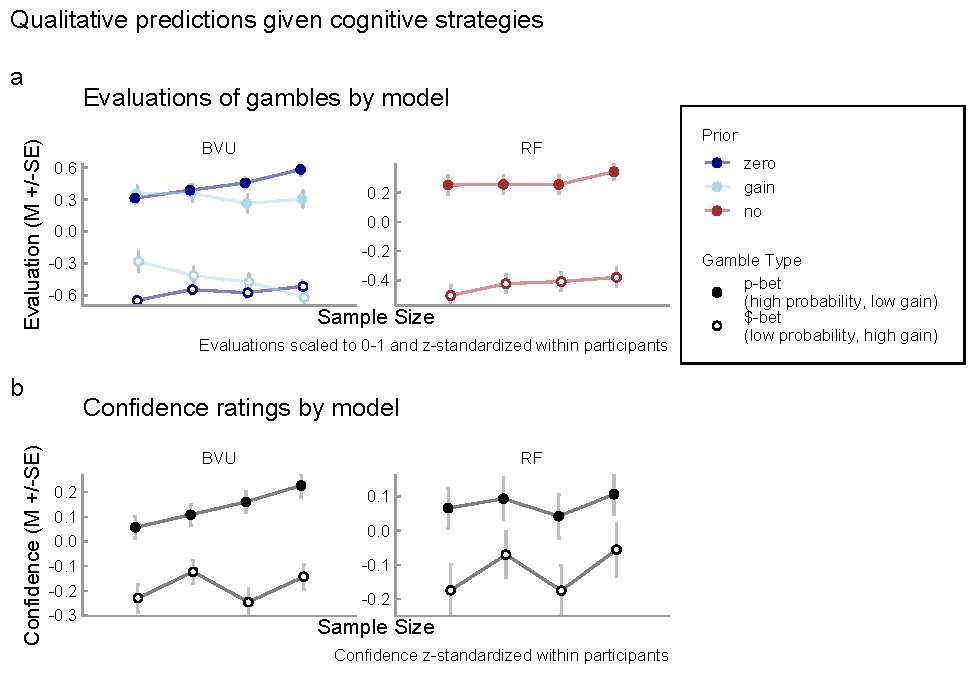
\includegraphics[width=.9\linewidth]{../figures/fig6-1} 

}

\caption{Mean evaluations by gamble type and best-fitting cognitive model and prior beliefs of the BVU model. \textit{BVU}$=$Bayesian value updating model, \textit{RF}$=$ Relative frequency model. Error bars indicate standard errors. Sample size categories see Table \ref{table:Lotteries}. Evaluations are scaled to 0-1 and z-standardized at the individual level.}\label{fig:fig6}
\end{figure}

\textit{Predictions about confidence.}
<<<<<<< Updated upstream
\added[id=jj]{The Bayesian model also predicts that people's confidence in their beliefs should increase the more evidence they gather. Thus in Bayesian learners, confidence should increase with growing sample size. The relative frequency model makes no predictions about confidence. To test this, we classified participants into Bayesian and relative-frequency learners based on the best-fitting model. Mean confidence ratings of Bayesian-type learners, z-standardized within participants, increased only slightly from the extra small sample size ($M=-0.07, SD=1.00$), to the small sample size ($M=0.01, SD=0.91$), medium sample size ($M=-0.01, SD=1.00$), and large sample size ($M=0.07, SD=1.00$, Figure \ref{fig:fig6}b), but statistical analyses showed that a linear regression model}\footnote{Regressing the (within-person z-standardized) confidence ratings on the predictors sample size category (coded as 1,2,3,4), gamble type, and winning model (BVU, RF), and interactions of the predictors, with a by-participant random intercept; categorical predictors were effects-coded to facilitate interpretation of interactions.}
\added[id=jj]{($M_1$) that includes the sample size as predictor described the data worse than an intercept-only model ($BF_{01}> 1000$).}
=======
\added[id=jj]{The Bayesian model also predicts that people's confidence in their beliefs should increase with more evidence they gather. Thus Bayesian learners' confidence is expected to increase with sample size. The relative frequency model makes no predictions about confidence. To test this, we classified participants into Bayesian and relative-frequency learners based on the best-fitting model. Mean confidence ratings of Bayesian-type learners, z-standardized within participants, increased only slightly from the extra small sample size ($M=-0.07, SD=1.00$), to the small sample size ($M=0.01, SD=0.91$), medium sample size ($M=-0.01, SD=1.00$), and large sample size ($M=0.07, SD=1.00$, Figure \ref{fig:fig6}b), but statistical analyses showed that a linear regression model}\footnote{Regressing the (within-person z-standardized) confidence ratings on the predictors sample size category (coded as 1,2,3,4), gamble type, and winning model (BVU, RF), and interactions of the predictors, with a by-participant random intercept; categorical predictors were effects-coded to facilitate interpretation of interactions.}
\added[id=jj]{($M_1$) that includes the sample size as predictor performed worse than an intercept-only model ($BF_{01}> 1000$).}

>>>>>>> Stashed changes

\end{document}
